\documentclass[a4paper,twoside,11pt, fleqn]{article}
\usepackage{a4wide,graphicx,fancyhdr,amsmath,amssymb}

%----------------------- Macros and Definitions --------------------------

\setlength\headheight{20pt}
\addtolength\topmargin{-10pt}
\addtolength\footskip{20pt}

\newcommand{\N}{\mathbb{N}}
\newcommand{\ch}{\mathcal{CH}}

\newcommand{\solution}[1]{\noindent{\bf Solution to Exercise #1:}}

\fancypagestyle{plain}{%
\fancyhf{}
\fancyhead[LO,RE]{\sffamily\bfseries\large technische universiteit eindhoven}
\fancyhead[RO,LE]{\sffamily\bfseries\large 2IN35 VLSI}
\fancyfoot[LO,RE]{\sffamily\bfseries\large department of mathematics and computer science}
\fancyfoot[RO,LE]{\sffamily\bfseries\thepage}
\renewcommand{\headrulewidth}{0pt}
\renewcommand{\footrulewidth}{0pt}
}

\pagestyle{fancy}
\fancyhf{}
\fancyhead[RO,LE]{\sffamily\bfseries\large technische universiteit eindhoven}
\fancyhead[LO,RE]{\sffamily\bfseries\large 2IN35 VLSI}
\fancyfoot[LO,RE]{\sffamily\bfseries\large department of mathematics and computer science}
\fancyfoot[RO,LE]{\sffamily\bfseries\thepage}
\renewcommand{\headrulewidth}{1pt}
\renewcommand{\footrulewidth}{0pt}

\def\addsquare#1{\tikz\node[draw]{#1};} 

%-------------------------------- Title ----------------------------------

\title{\vspace{-\baselineskip}\sffamily\bfseries Assignment 3}
\author{
	Rick Veens \qquad Studentno: 0912292\\
	\texttt{r.veens@student.tue.nl}
	\and
	Barry de Bruin \qquad Studentno: -\\
	\texttt{-@student.tue.nl}
}

\date{\today}

\setlength\parindent{0pt}

%--------------------------------- Text ----------------------------------

\begin{document}
\maketitle
\newpage

\section*{Lab assignment 3a}
\subsection*{1. Requirements}
The assignment is to design and implement a FIR filter named filter that:
\begin{enumerate}
\item Uses as little resources as possible and is maximally sequential. In particular at most 1
multiplier may be used.
\item Conforms to the 4-phase asynchronous protocol for both input and output.
\item Can run at a clock frequency of 100 Mhz.
\item Honors changes in the coefficients (after a finite delay).
\item May produce a finite length interval of start-up noise
\end{enumerate}

\subsubsection*{1.1 Analysis of requirements}
The FIR filter should make use of only one DSP-unit, since the internal clock frequency is significantly higher than the expected sample rate. Furthermore the coefficients should not be buffered but must be connected as wires instead of buffering them in registers. This ensures that requirement 1 and 4 can be satisfied. For requirement 3, the clock frequency should be at least 100MHz, which will be checked in the post-synthesis report. Lastly, the asynchronous ack/req protocol will be used since there needs to be some synchronization between the testbench (44.1KHz sample rate) and the filter (100MHz sample rate).


\subsection*{2. System architecture}
Figure one shows the global architecture of the FIR filter. 
\begin{figure}[h]
	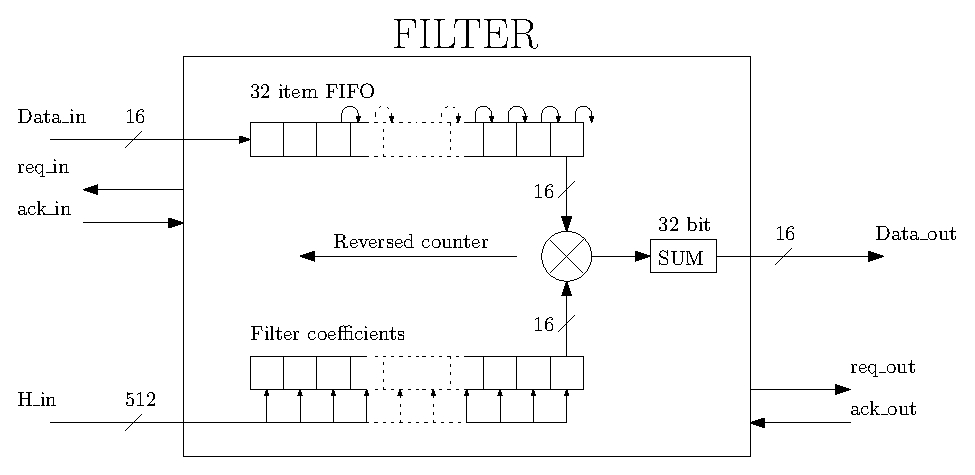
\includegraphics[scale = 1]{Images/3a_blockdiagram}
    \caption{System overview}
\end{figure}

Unlike the FIR filter of lab2, the filter has only one tap. After each clock edge the multiplier/accumulator will multiply a sample that is stored in the memory with it's corresponding filter coefficient. An index makes sure that this operation moves through the FIFO in 32 clock cycles. The index sample is also shifted one place to the right. After 32 cycles the last tap has  been calculated and the first place in the FIFO is empty. The system will output the calculated sample, and request a new data item, which will be put on the first index.\\ 

The whole procedure will then restart.
\subsection*{4. Design choices}

\subsection*{5. Functional correctness}
all requirements?

\subsection*{6. Resource usage}
Table 1 summarizes the resources used by the FIR filter. This list is obtained by running the synthesis step in Xilinx ISE and extracted from the \textit{Summary} and \textit{Device Utilization} report.
\begin{table}[h]
\begin{tabular}{|l|l|l|l|}
\hline
\textbf{Resource} & \textbf{Available} & \textbf{Utilized} & \textbf{Percentage utilized}\\
\hline
Flip Flops	& 54576 & 1064 	& 1\%\\
Slice LUTs 	& 27288 & 527 	& 1\%\\
DSP48A1s	& 58 	& 1 	& 1\%\\
BRAM		& 116 	& 0 	& 0\%\\
Bonded IOBs	& 218 	& 40 	& 18\%\\
\hline
\end{tabular}
\caption{General resource usage overview}
\end{table}

The number of flipflops used in the design are:
\begin{align*}
Total_{\#reg}	&= sum + data + coef + cnt + state + flow control\\
			&= 32 + 16\cdot 32 + 32\cdot 16 + 5 + 1 + 2\\
			&= 1064
\end{align*}
This number matches the synthesis result.\\

There is only one DSP unit used, since the filter is fully sequential. This results in a significant resource reduction since the DSP units are quite expensive. According to the summary report, almost all slice LUTs are used for logical ports. They are used to model the 5 bit counter that counts up to 32. The number of Bonded IOB's represents the number of pins used on the FPGA. These pins are occupied by the clk, rst, h\_in, h\_enabled,  $2\cdot 16$ input and output pins and 2 pairs of ack/req pins.\\

Furthermore some additional resources are used to enable the possibility to shift the data in the FIFO every clock cycle.

\subsection*{7. System throughput and latency}
The minimum sample time estimation is extracted from the \textit{Synthesis report} under \textit{Timing Report}.\\

   \textit{Minimum period: 8.421ns (Maximum Frequency: 118.750MHz)\\
   Minimum input arrival time before clock: 6.274ns\\
   Maximum output required time after clock: 4.350ns}\\

This time is equal to the largest critical path (the calculation of the tap is the critical path in this design).\\

After doing the placement and routing step, we will get a more accurate measurement of the maximum achievable throughput. These measurements can be found in the \textit{Advanced Post-PAR static timing report} under \textit{Timing summary}:\\

   \textit{Minimum period:   9.695ns   (Maximum frequency: 103.146MHz)\\
   Minimum input required time before clock:  10.637ns\\
   Maximum output delay after clock:  11.028ns}\\

Since the minimum period is not the maximum delay, we should take the largest 
delay as a definition for the maximum clock frequency. This will yield us a maximum system frequency of:\\

$F_{max} = \frac{1}{T_{max delay}} = \frac{1}{11.028ns} = 90.6MHz$\\

This frequency is significantly less than the expected maximum sample rate (or clock frequency) retrieved from the synthesis. This is expected due to the fact that the place and route report also takes the physical layout delays into account, and the synthesis does not. This can be improved by placing a simple buffer at the output of the filter:\\

Post-PAR static timing summary after improvement:\\
\textit{Minimum period:   9.712ns{1}   (Maximum frequency: 102.965MHz)\\
   Minimum input required time before clock:   8.630ns\\
   Maximum output delay after clock:   8.824ns}\\

Therefore our final frequency will be above 100MHz.


\subsection*{8. Simulation results}
Time en FFT plot


\newpage
\section*{Lab assignment 3b}
\subsection*{1. Requirements}
The specific requirements for the strength reduced FIR filter are:
\begin{enumerate}
\item The design may use at most 3 multipliers.
\item Conforms to the 4-phase asynchronous handshake protocol for both input and output.
\item Can run at a clock frequency of 100 Mhz.
\item Should have about 4 times the sample frequency as the sequential implementation.
\item Honors changes in the coefficients (after a finite delay).
\item May produce a finite length interval of start-up noise.
\end{enumerate}


\newpage
\section*{Comparison between two filters}
In your final report, compare the output signals of the strength reduced filter with the output of the sequential filter, by generating a difference signal for a representative subset of
samples. Make sure you align the outputs correctly, because the amount of start-up noise of
the 2 implementations may differ. If the difference signal is non-zero, explain the differences.
Further reporting guidelines are on the course’s website.

\newpage
\section*{Appendix}
all verilog code



\end{document}
